\chapter{Durchführung}\label{cha:durchfuehrung}
\section{Vorbereitung}\label{sec:vorbereitung}
\subsection{Auswahl der Umgebung und Höhe}\label{sub:auswahlUmgebung}
Um das Experiment durchzuführen müssen verschiedene Vorbereitungen vorgenommen werden. Zuerst muss der Ort ausgewählt werden. Um das Experiment möglichst erfolgreich und präzise zu halten, sollte es in einem möglichst dunklen Raum durchgeführt werden. Für diese Arbeit wurde die Dunkelkammer (Zimmer G10) der Kantonsschule am Burggraben zur Verfügung gestellt. Ein weiterer Punkt der Vorbereitung ist der Untergrund, auf dem das Experiment steht. Im Experimentierkasten kommen Verlängerungsstäbe mit, die dazu dienen das Experimentieren angenehmer zu machen. Das Problem mit diesen Stäben ist, dass sie Vibrationen nicht weghalten und das Experiment sehr anfällig für diese ist. In dieser Arbeit wurde die Plattform auf ein Holzklotz gelegt, damit das Experiment auf Augenhöhe ist bei gestrecktem Rücken. Die Plattform sollte gerade stehen. Das kann man mit der Wasserwaage auf der Plattform kontrollieren. Falls die Plattform schräg sein sollte, kann man mit den veränderbaren Füssen die Plattform ausebenen. Mit diesem Holzklotz hatte das Experiment einen festen Untergrund und war somit bereit für das Einstellen des optischen System. 

\subsection{Kondensatorenabstand messen}\label{sub:kondensatorenabstand}
Der nächste Schritt für die Vorbereitung ist das Messen des Abstandes zwischen den beiden Kondensatoren. Das Wichtige bei diesem Schritt ist, dass die Spannung abgeschaltet ist. Zuerst wird das Gehäuse der Betrachtungskammer abgenommen. Danach wird die obere Platte vorsichtig weggenommen und die darunter liegende Platte aus Kunststoff auch. Im Experimentierkasten befindet sich eine Schieblehre. Damit misst man die Dicke der Kunststoffplatte. Wichtig ist, dass man am inneren Rand der Platte misst und nicht am äusseren, da der äussere Rand ein Bisschen dicker ist. Jetzt kann der Wert direkt abgelesen und notiert werden. 

\section{Das optische System ausrichten}\label{sec:optischesSystem}
\subsection{Das Betrachtungsfernrohr fokussieren}
Die Betrachtungskammer sollte jetzt wieder zusammengebaut werden, das Gehäuse aber noch nicht. Auf der Platte soll der Fokussierdraht abgeschraubt werden und Vorsichtig in das Loch in der Mitte der oberen Kondensatorenplatte eingeführt werden. Danach muss die Halogenlampe angeschlossen werden. Dafür muss der Stecker des 12 V DC Transformator an die Lampe angeschlossen werden, dann sollte die Lampe leuchten. Jetzt muss zuerst das Fadenkreuz in Fokus gesetzt werden. Dafür muss man den Fadenkreuz-Fokussierring drehen bis man das komplette Gitter scharf sieht. Dann sollte man den Draht anschauen durch das Betrachtungsfernrohr und den Tröpfchen-Fokussierring solange drehen bis man den Draht scharf sehen kann. 

\subsection{Die Halogenlampe einstellen}\label{sub:Halogenlampe}
Mit dem horizontalen Einstellknopf der Halogenlampe soll das Licht auf der horizontalen Ebene richtig fokussiert werden. Damit das Licht am besten fokussiert ist, muss der rechte Rand des Drahtes am hellsten sein. Das heisst, im grössten Kontrast zur linken Seite des Drahtes stehen. Mit dem vertikalen Einstellungsknopf muss das Licht auf der Mitte des Gitters / Fadenkreuz am besten zu sehen sein. Wenn alles fertig eingerichtet ist, sollte der Fokussierdraht wieder in die Vertiefung in der Platte verschraubt werden.

\section{Funktionen der Steuerung}\label{sec:funktionen}
\subsection{Der Ionisationsquelle Schalter}\label{sub:ionisationquelle}
Der Schalter für die Ionisation hat 3 verschiedene Positionen. Die An-Position, die Aus-Position und die Tröpfchensprüh-Position. Wenn der Schalter auf der Aus-Position ist, wird die Ionisationsquelle komplett abgeschirmt und es können keine Alphateilchen in die Kammer gestrahlt werden. Bei der An-Position ist dieser Schirm nicht mehr da und die Öltröpchen können angestrahlt werden. Die dritte Position, die Tröpfchensprüh-Position, muss geschaltet werden, wenn die Ölrtöpchen eingesprüht werden. Bei dieser Position öffnet sich ein kleines Loch in der Kammer, damit die Luft ausströmen kann, wenn das Öl eingesprüht wird.

\begin{figure}[ht]
	\begin{center}
		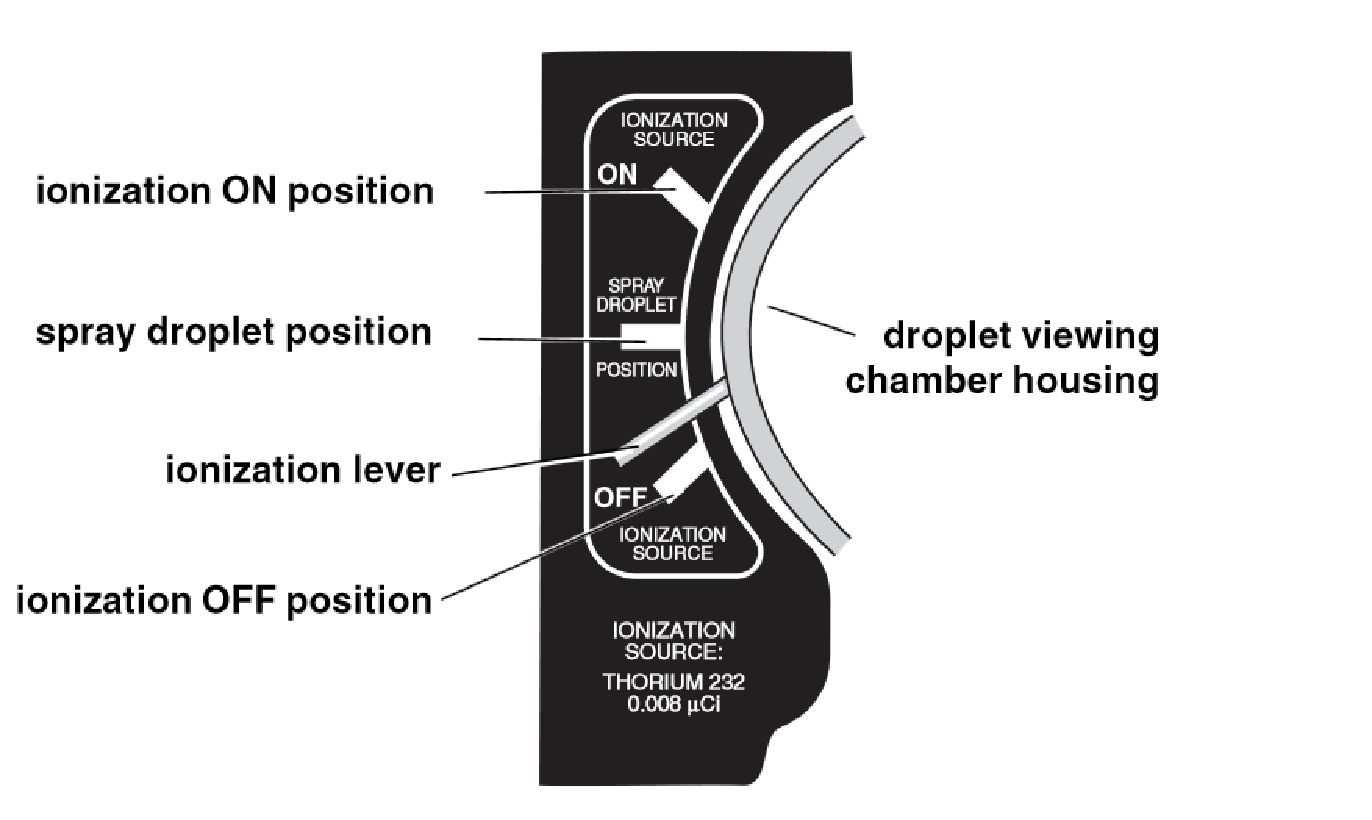
\includegraphics[scale=0.5]{bilder/pdf/Schalterfunktionen.pdf}
		\caption{Schalterpositionen der Ionisationsquelle}
		\label{fig:Schalterpositionen}
	\end{center}
\end{figure}

\subsection{Kondensatorenspannung Schalter}\label{sub:Spannungsschalter}
lorem ipsum